\section{Results}\label{sec:results}

% TODO: I'm aware the I need to refine the text. Tips are welcomed :) 
% In this section we present the results of the three experiments presented in Section~\ref{sec:experiments}. We present them one by one to facilitate the analysis.

\subsection*{Experiment 1: evolution during training}

Figure~\ref{fig:results:exp1:evolution} shows the evolution of the \textit{best reward} and the \textit{accumulated reward} per episode (representing the quality of the neural architectures), as well as the \textit{episode length} (in a chain-structured network this represents the number of layers). We observe that, in the first environment (\textit{omniglot}), our deep meta-RL agent performs worse than \textsc{DeepQN}. Nevertheless, in the second and third environments (\textit{vgg\_flower}, \textit{dtd}), the agent performs better than the baselines from the very first steps, and more consistently through all episodes (showing less variance). \textsc{DeepQN} only catches up after many more episodes.

Figure~\ref{fig:results:entropy} shows the entropy of the policy during training over the different environments, which in the A2C algorithm is related to the level of exploration by the agent (more exploration leads to high entropy). In the first environment, our agent explores the environment for a significant number of time-steps, which translates to the slow increase observed in Figure~\ref{fig:results:exp1:evolution:a}. In the second environment, the exploration drops down quickly, except for a short period with increased exploration (time-steps 9005 to 12005). In the last and hardest environment, the agent re-explores the environment to adapt its strategy, leading to a reduction of the episode length (depth of the networks) and, consequently, the accumulated reward does not appear to increase due to the shorter episodes. We believe that exploration causes the drops in episode length in \textit{vgg\_flower} and \textit{dtd} (Figures~\ref{fig:results:exp1:evolution:e} and~\ref{fig:results:exp1:evolution:h}).

In Figure~\ref{fig:results:exp1:actions}, the proportion of the actions performed by the agent during training is shown. We see that it deployed different strategies per environment. Specifically, we note the changes in proportion for actions \textsc{A0} (\textit{convolution} with a kernel of size 1),  \textsc{A3} (\textit{max-pooling} with pool size of 2), and \textsc{A7} (the \textit{terminal} state) when the environment switched from \textit{vgg\_flower} to \textit{dtd}, suggesting that the agent preferred different layers and depth according to the dataset.

Finally, Table~\ref{tab:results:times} shows the running times per environment for each RL algorithm. Here, we do not observe significant differences considering that once transferred, the policy of the deep meta-RL agent designs deeper and more costly networks, as observed in Figures~\ref{fig:results:exp1:evolution:e} and~\ref{fig:results:exp1:evolution:h}.

\begin{figure}[ht]
\centering
\begin{subfigure}{.33\textwidth}
  \centering
      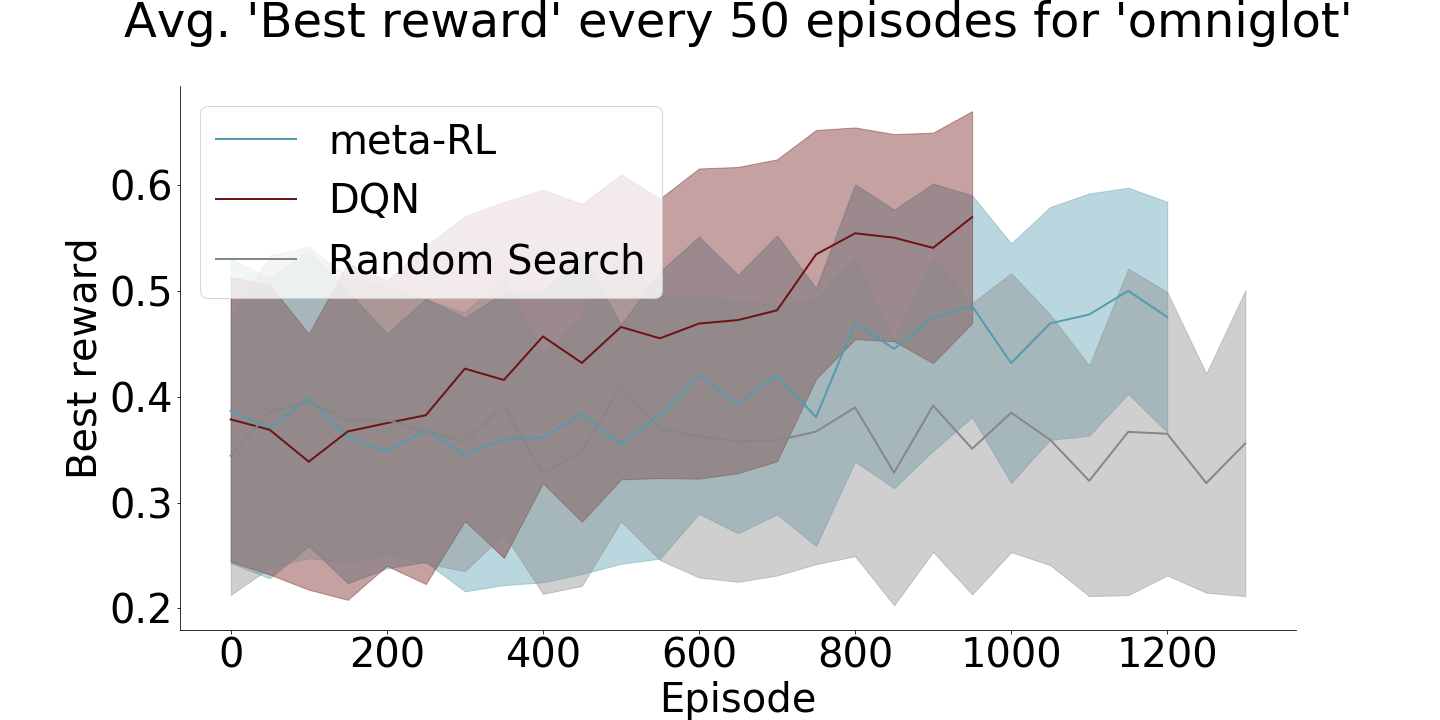
\includegraphics[width=\linewidth]{imgs/chained/average-best_reward-omniglot.png}
  \caption{}
  \label{fig:results:exp1:evolution:a}
\end{subfigure}%
\begin{subfigure}{.33\textwidth}
  \centering
      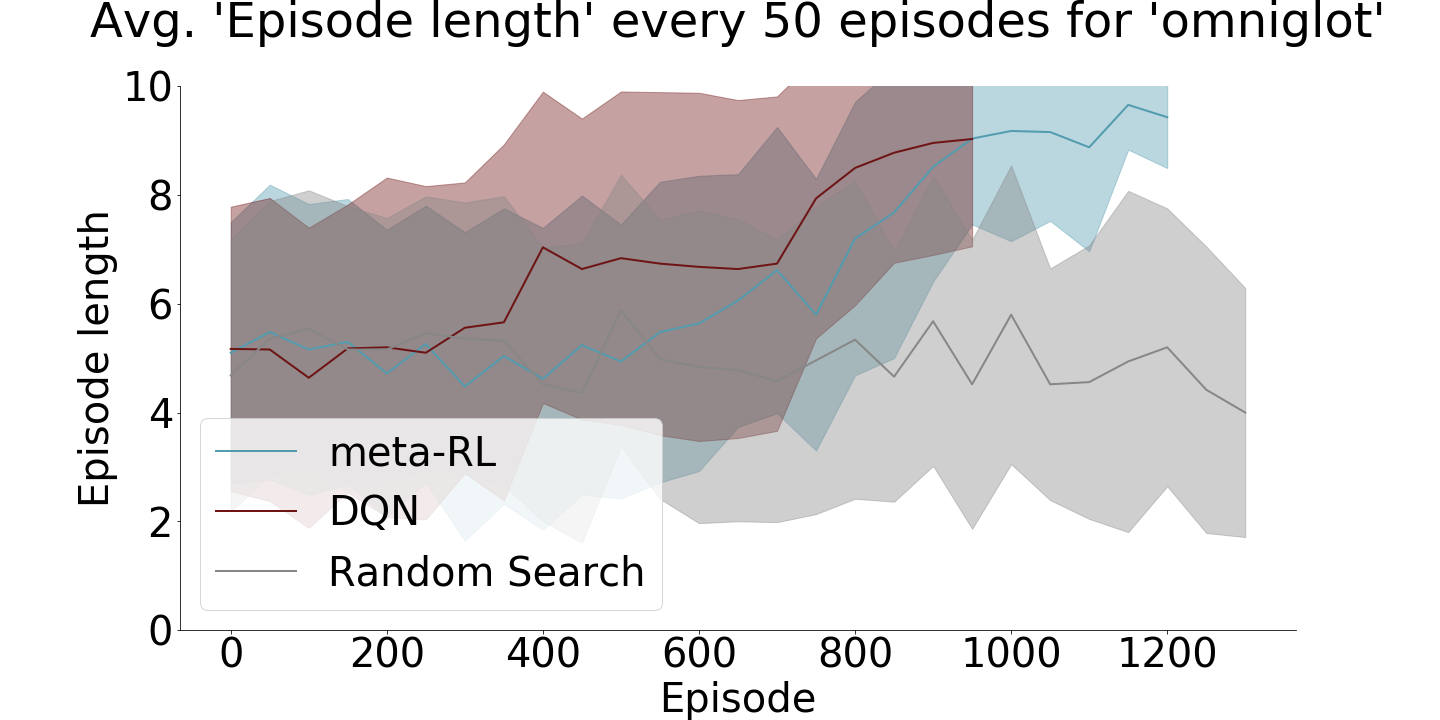
\includegraphics[width=\linewidth]{imgs/chained/average-ep_length-omniglot.png}
  \caption{}
  \label{fig:results:exp1:evolution:b}
\end{subfigure}%
\begin{subfigure}{.33\textwidth}
  \centering
      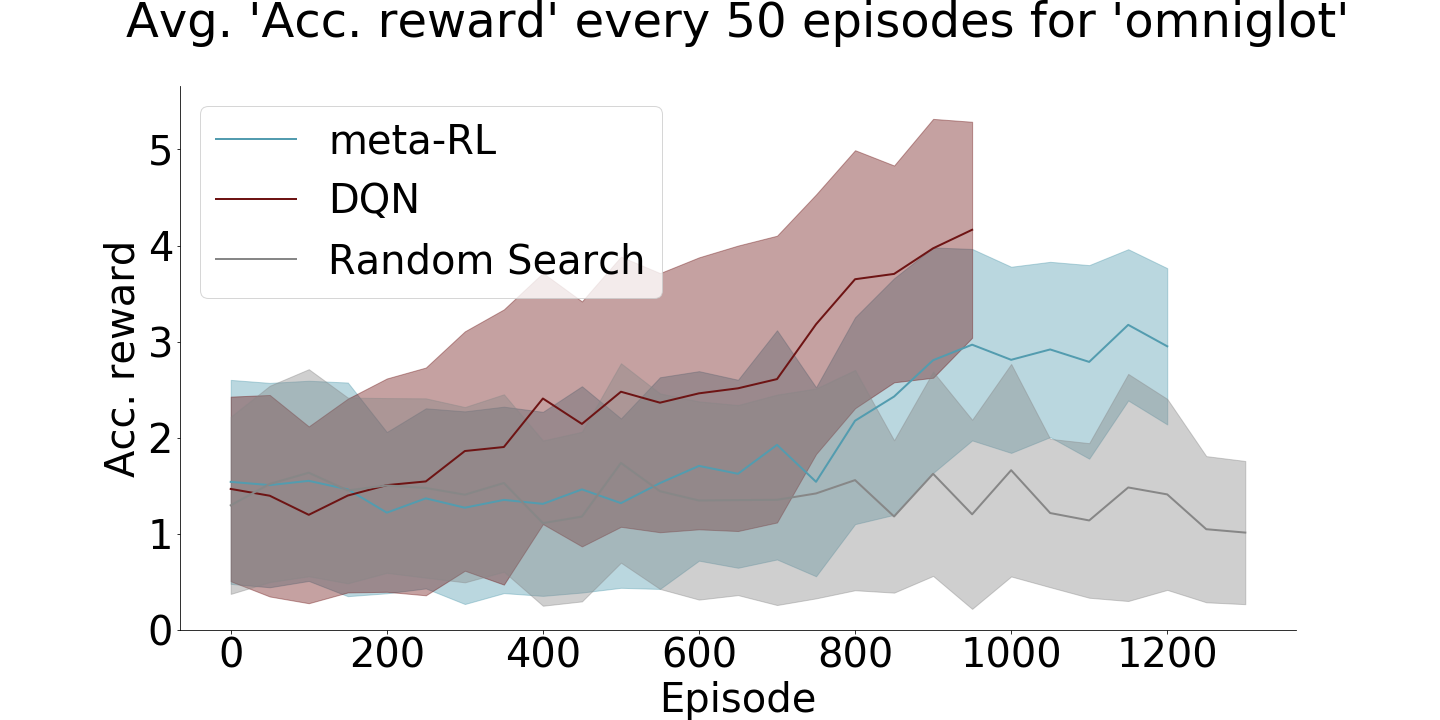
\includegraphics[width=\linewidth]{imgs/chained/average-acc_reward-omniglot.png}
  \caption{}
\label{fig:results:exp1:evolution:c}
\end{subfigure}
\begin{subfigure}{.33\textwidth}
  \centering
      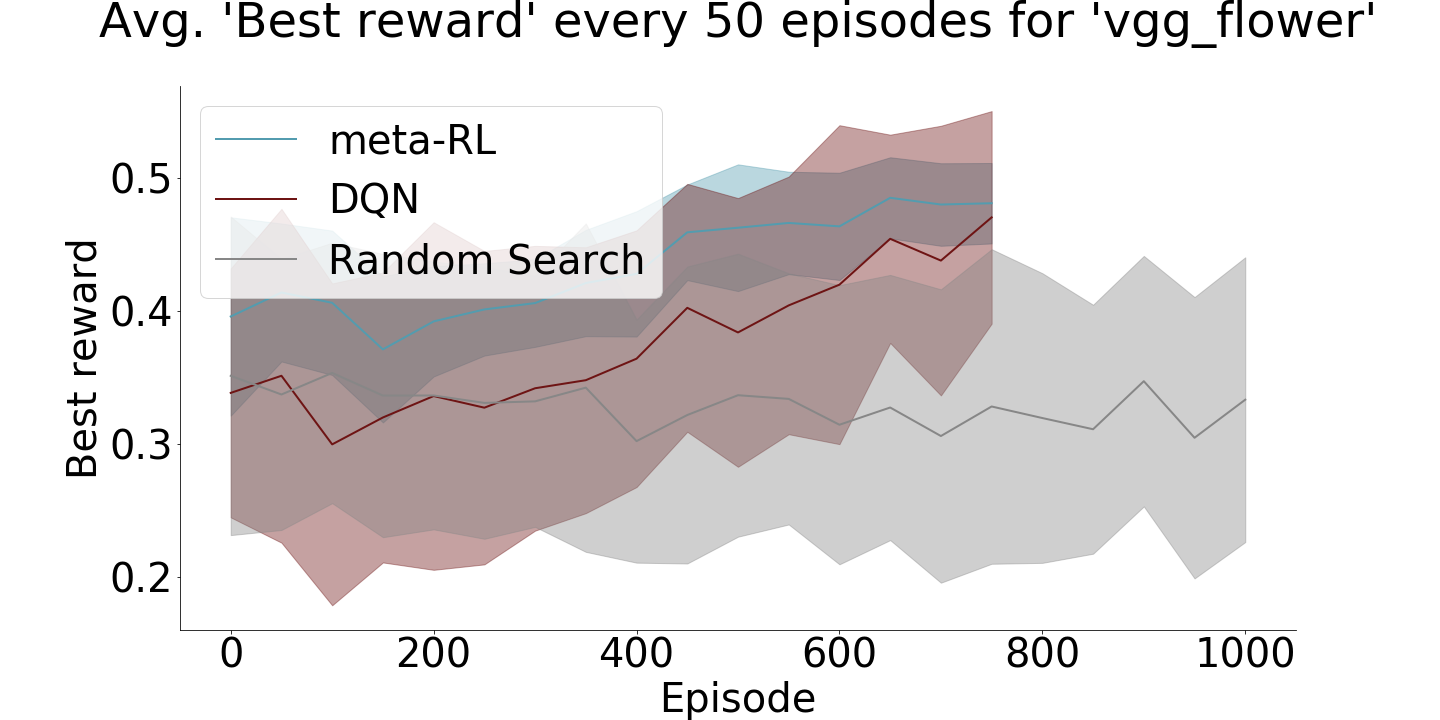
\includegraphics[width=\linewidth]{imgs/chained/average-best_reward-vgg_flower.png}
  \caption{} 
\label{fig:results:exp1:evolution:d}
\end{subfigure}%
\begin{subfigure}{.33\textwidth}
  \centering
      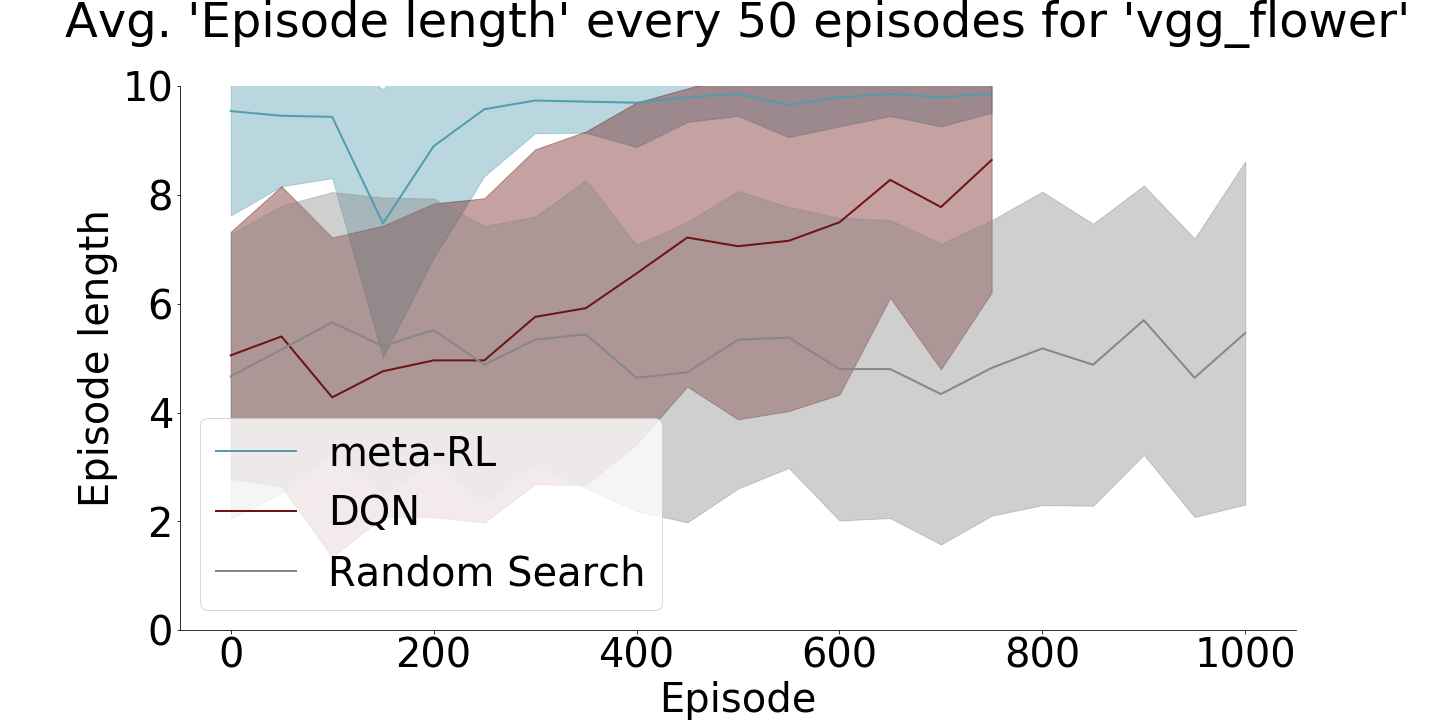
\includegraphics[width=\linewidth]{imgs/chained/average-ep_length-vgg_flower.png}
  \caption{}
\label{fig:results:exp1:evolution:e}
\end{subfigure}%
\begin{subfigure}{.33\textwidth}
  \centering
      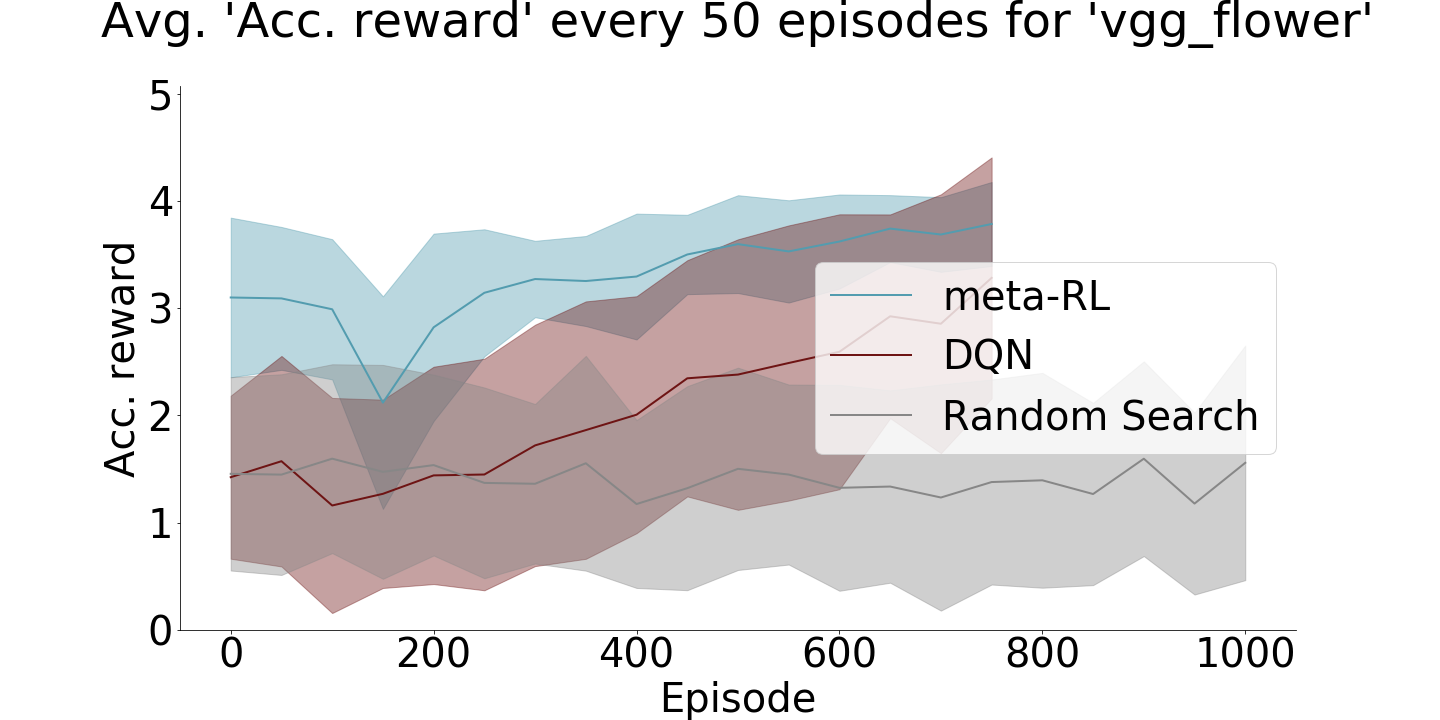
\includegraphics[width=\linewidth]{imgs/chained/average-acc_reward-vgg_flower.png}
  \caption{} 
\label{fig:results:exp1:evolution:f}
\end{subfigure}
\begin{subfigure}{.33\textwidth}
  \centering
      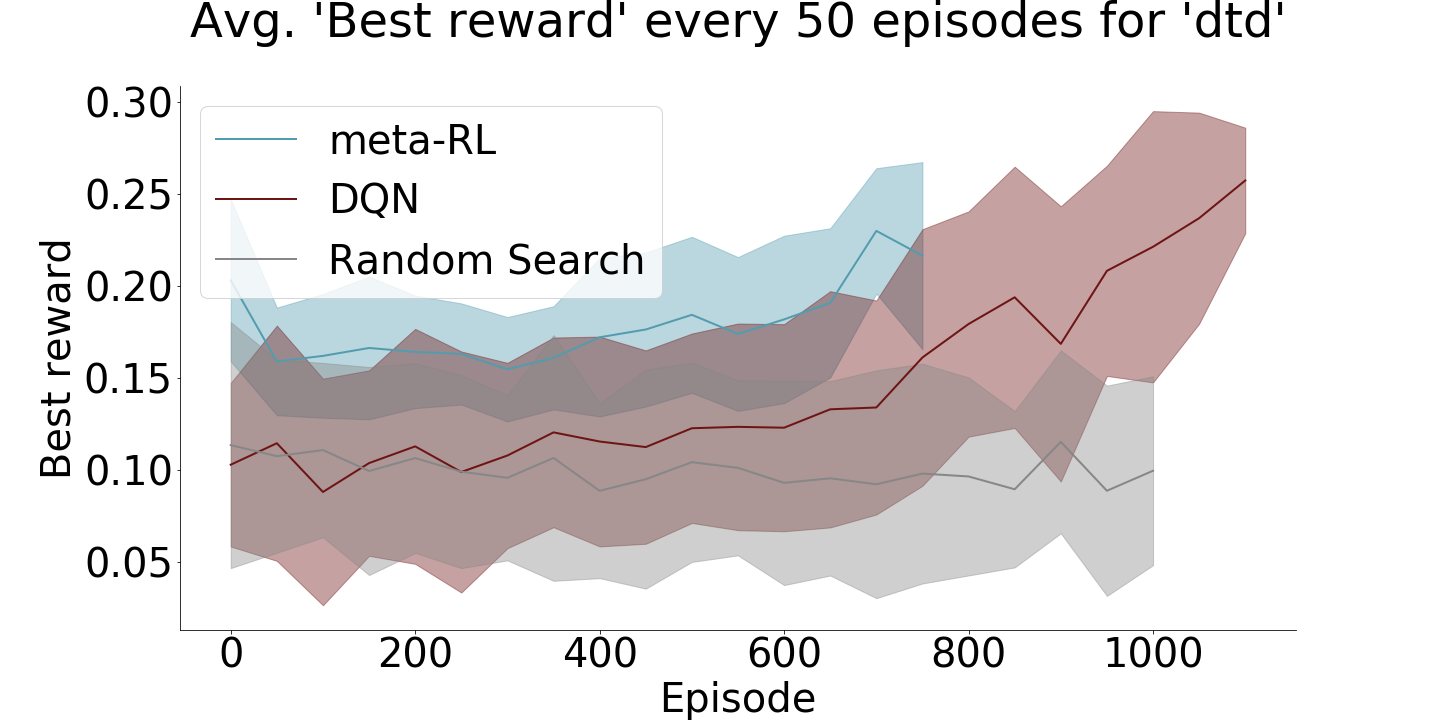
\includegraphics[width=\linewidth]{imgs/chained/average-best_reward-dtd.png}
  \caption{}
\label{fig:results:exp1:evolution:g}
\end{subfigure}%
\begin{subfigure}{.33\textwidth}
  \centering
      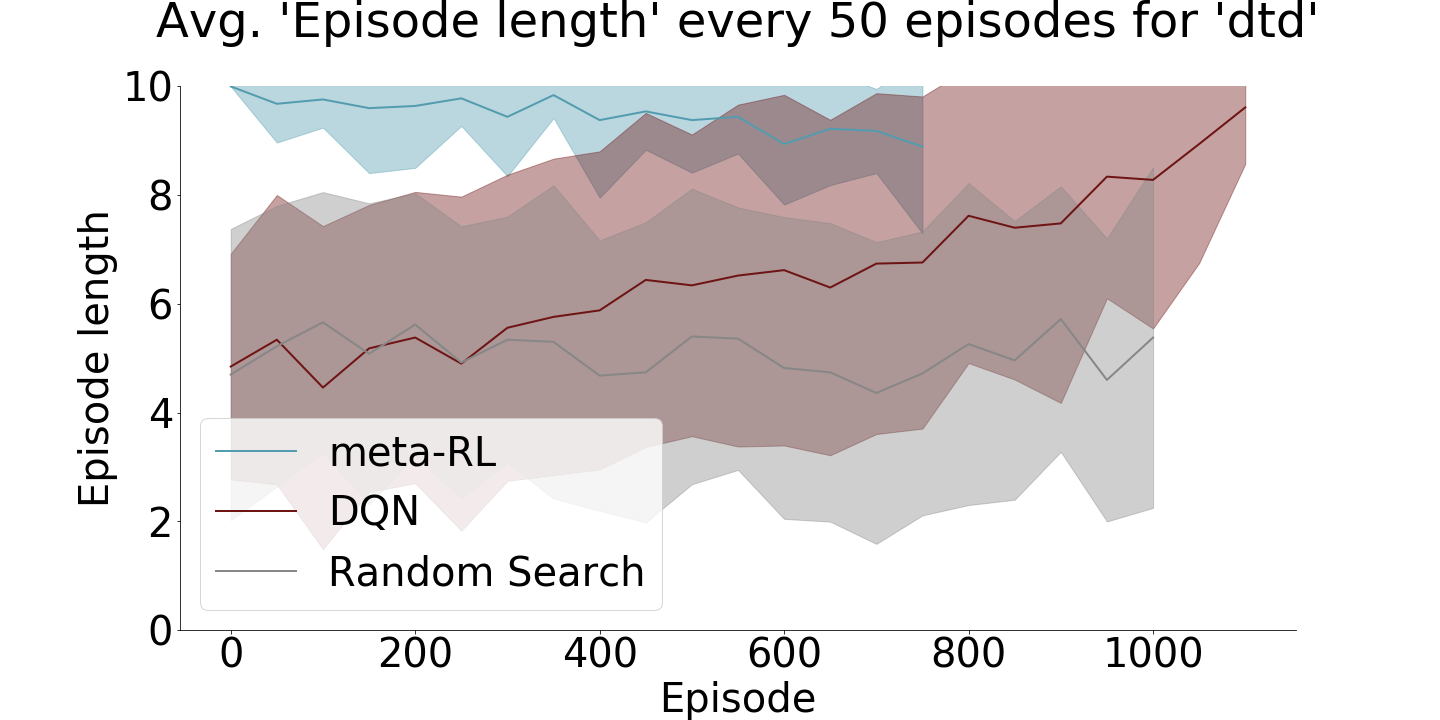
\includegraphics[width=\linewidth]{imgs/chained/average-ep_length-dtd.png}
  \caption{} 
\label{fig:results:exp1:evolution:h}
\end{subfigure}%
\begin{subfigure}{.33\textwidth}
  \centering
      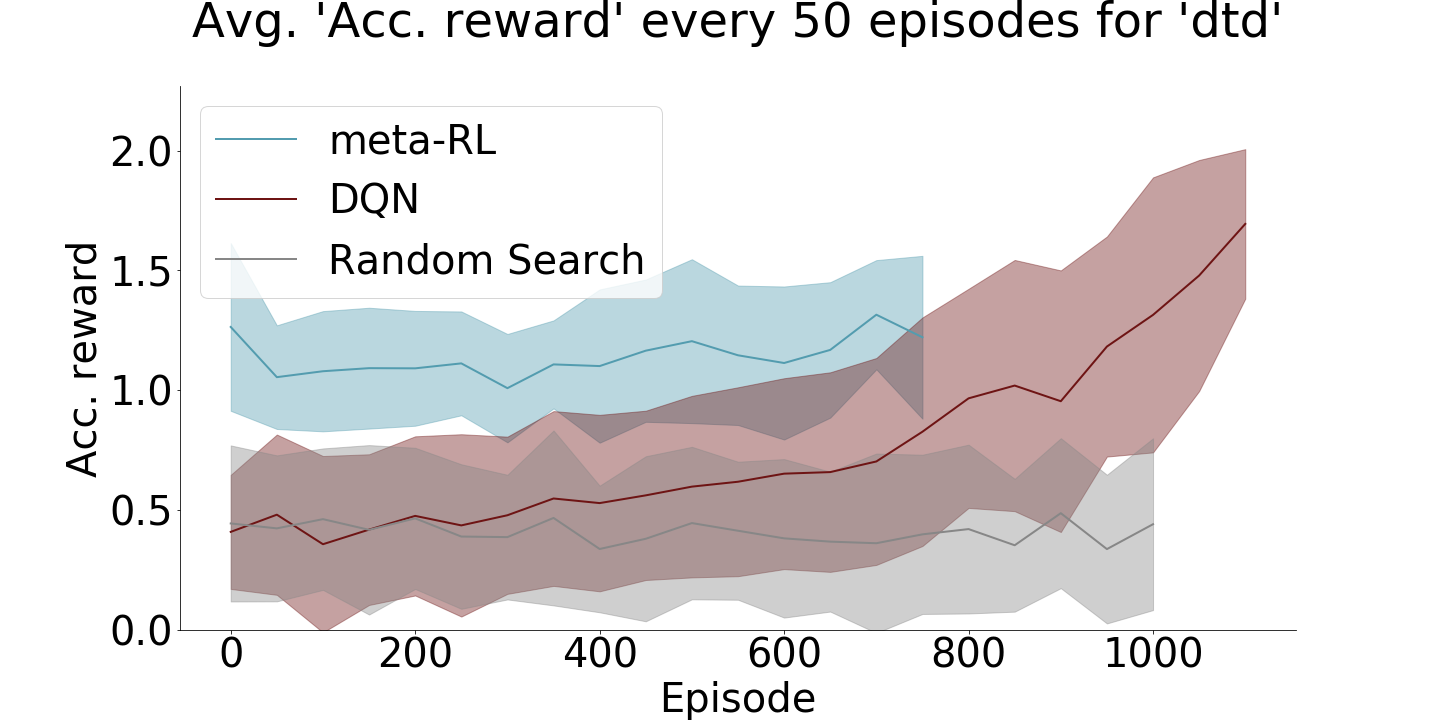
\includegraphics[width=\linewidth]{imgs/chained/average-acc_reward-dtd.png}
  \caption{} 
\label{fig:results:exp1:evolution:i}
\end{subfigure}
\caption{Evolution of training episodes through time from different perspectives, showing the means and $\pm 1$ standard deviations for every 50 episodes. Since the different techniques can build networks of different depths per episode, but are bound by the same $t_{max}$, the number of episodes executed per environment may differ.}
\label{fig:results:exp1:evolution}
\vspace{-0.5cm}
\end{figure}


\begin{figure}[ht]
\centering
    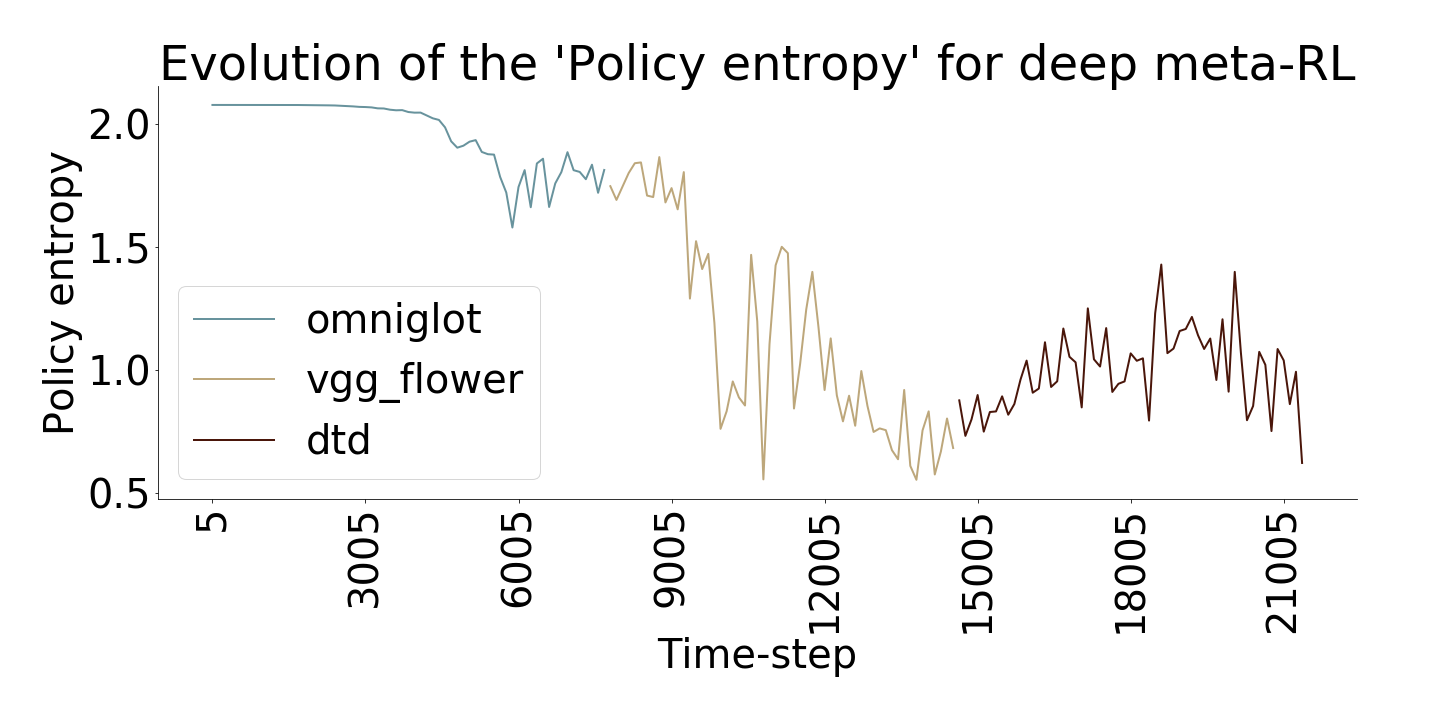
\includegraphics[width=0.65\linewidth]{imgs/chained/entropy.png}
\caption{Policy entropy through environments}
\label{fig:results:entropy}
% \vspace{-0.5cm}
\end{figure}

\begin{figure}[ht]
\centering
    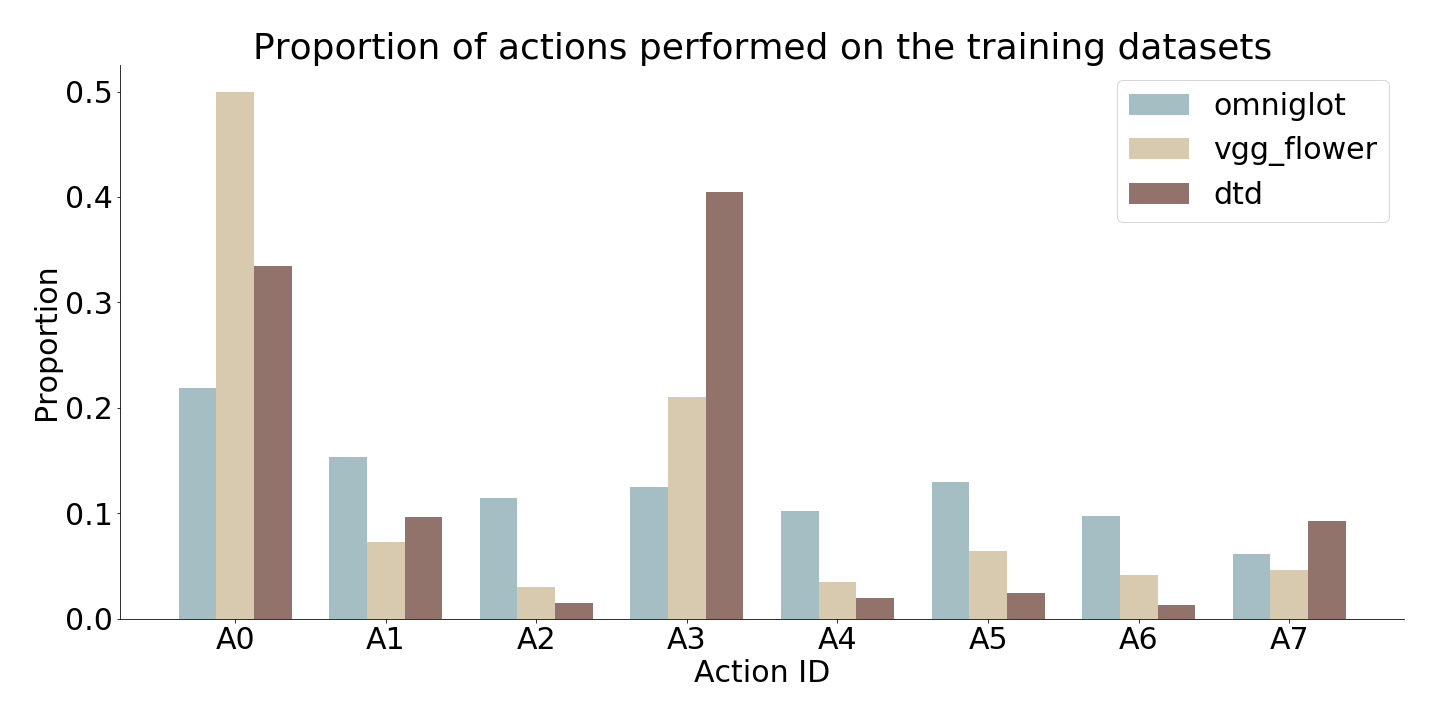
\includegraphics[width=0.65\linewidth]{imgs/chained/actions-dist-training.png}
\caption{Proportion of actions performed by the agent per dataset. The labels in the x-axis match the IDs in Table~\ref{tab:methodology:rl:as}.}
\label{fig:results:exp1:actions}
% \vspace{-0.5cm}
\end{figure}


\begin{table}[ht]
\centering
\begin{tabular}{@{}ccc@{}}
\toprule
Dataset     & Deep meta-RL & DQN         \\ \midrule
omniglot    & 11 days 9h   & 6 days 14h    \\
vgg\_flower & 7 days 23h   & 5 days 15h     \\
dtd         & 6 days 17h   & 6 days 4h      \\ \midrule
Total       & 26 days 1h   & 18 days 9h    \\ \bottomrule
\end{tabular}
\caption{Running times per dataset during training. All experiments ran on a single NVIDIA Tesla K40m GPU.}
\label{tab:results:times}
\end{table}


% \end{minipage}


\subsection*{Experiment 2: evaluation of the policy}

The results of replaying the learned policy on completely new datasets are displayed in Figure~\ref{fig:results:exp2:evolution}, and the corresponding runtimes are shown in Table~\ref{tab:results:exp2:times}. They show that the agent immediately finds a good solution (with a deep network), and rewards remain consistent; however, it does not improve over time, which warrants further study (see Section~\ref{sec:conclusions}). Moreover, the strategy deployed by the agent is not different on each dataset, as it is observed in Figure~\ref{fig:results:exp2:actions}. We confirm that the strategies are not significantly different by performing a Wilcoxon signed-rank test with the null hypothesis that the two related paired samples come from the same distribution. The output is a $\text{p-value}=0.48$ with 95\% confidence.

\begin{figure}[ht]
\centering
\begin{subfigure}{.33\textwidth}
  \centering
      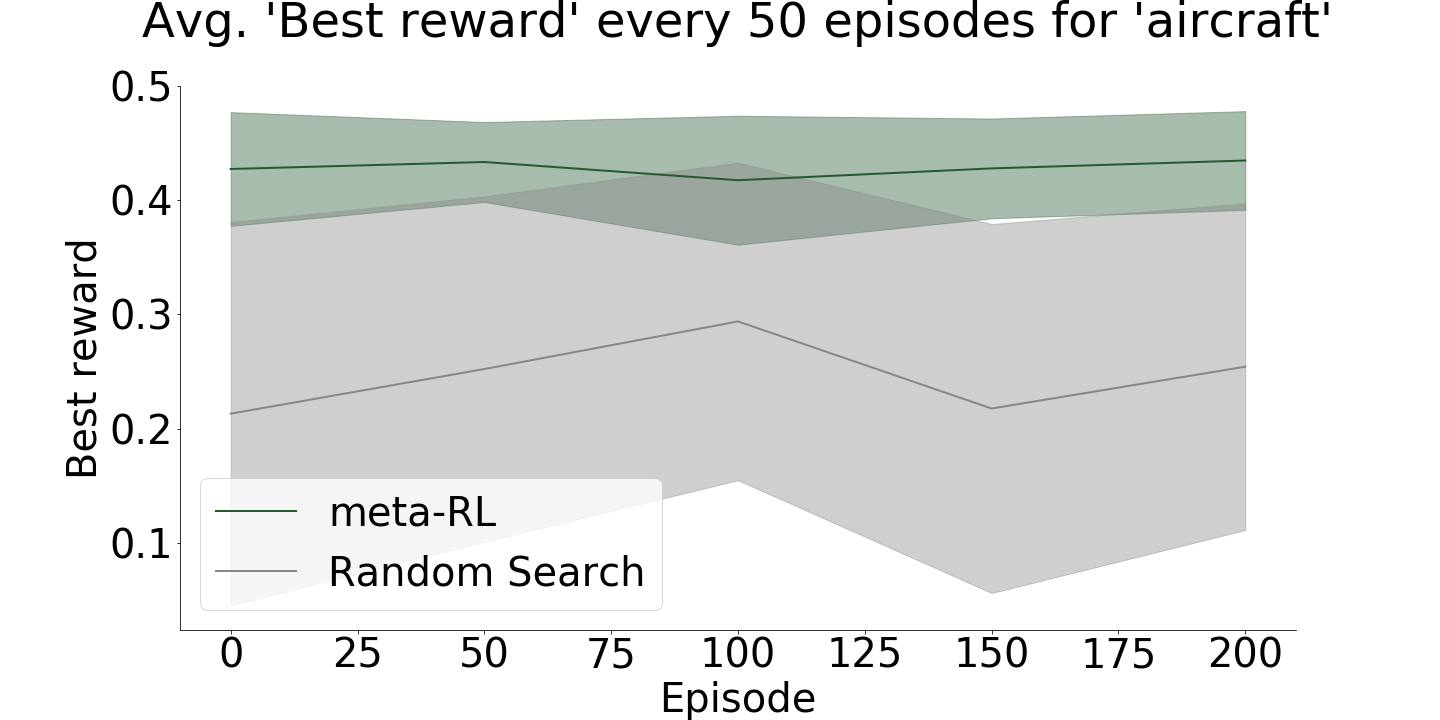
\includegraphics[width=\linewidth]{imgs/chained/average-best_reward-aircraft.png}
  \caption{}
  \label{fig:results:exp2:evolution:a}
\end{subfigure}%
\begin{subfigure}{.33\textwidth}
  \centering
      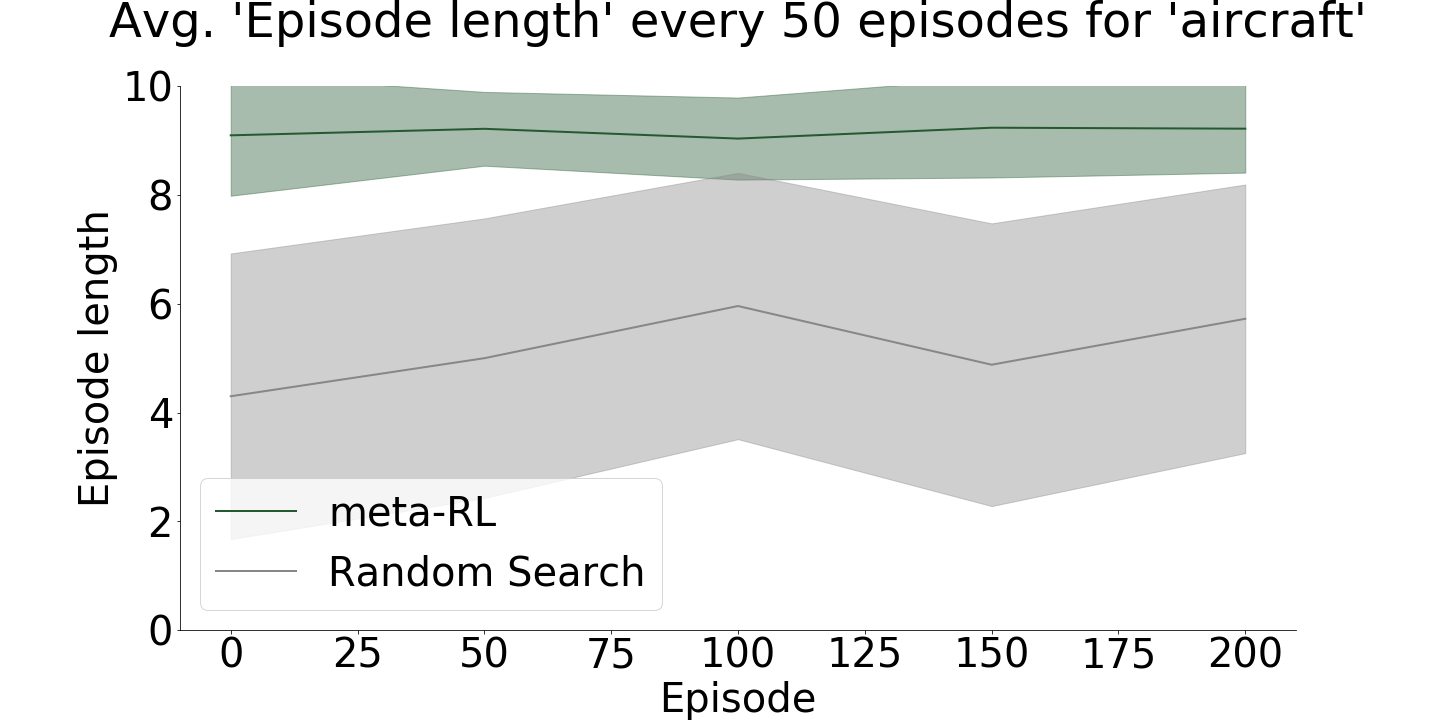
\includegraphics[width=\linewidth]{imgs/chained/average-ep_length-aircraft.png}
  \caption{}
  \label{fig:results:exp2:evolution:b}
\end{subfigure}%
\begin{subfigure}{.33\textwidth}
  \centering
      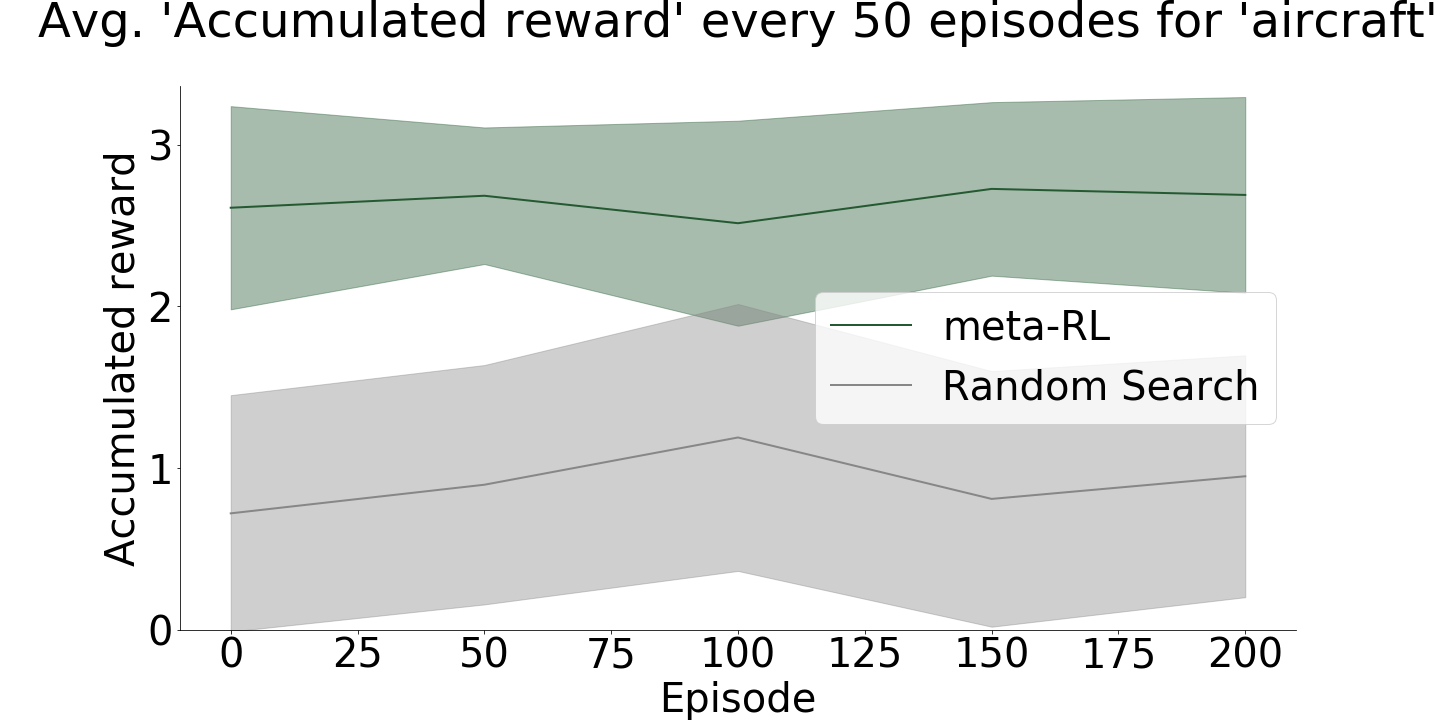
\includegraphics[width=\linewidth]{imgs/chained/average-acc_reward-aircraft.png}
  \caption{}
\label{fig:results:exp2:evolution:c}
\end{subfigure}
\begin{subfigure}{.33\textwidth}
  \centering
      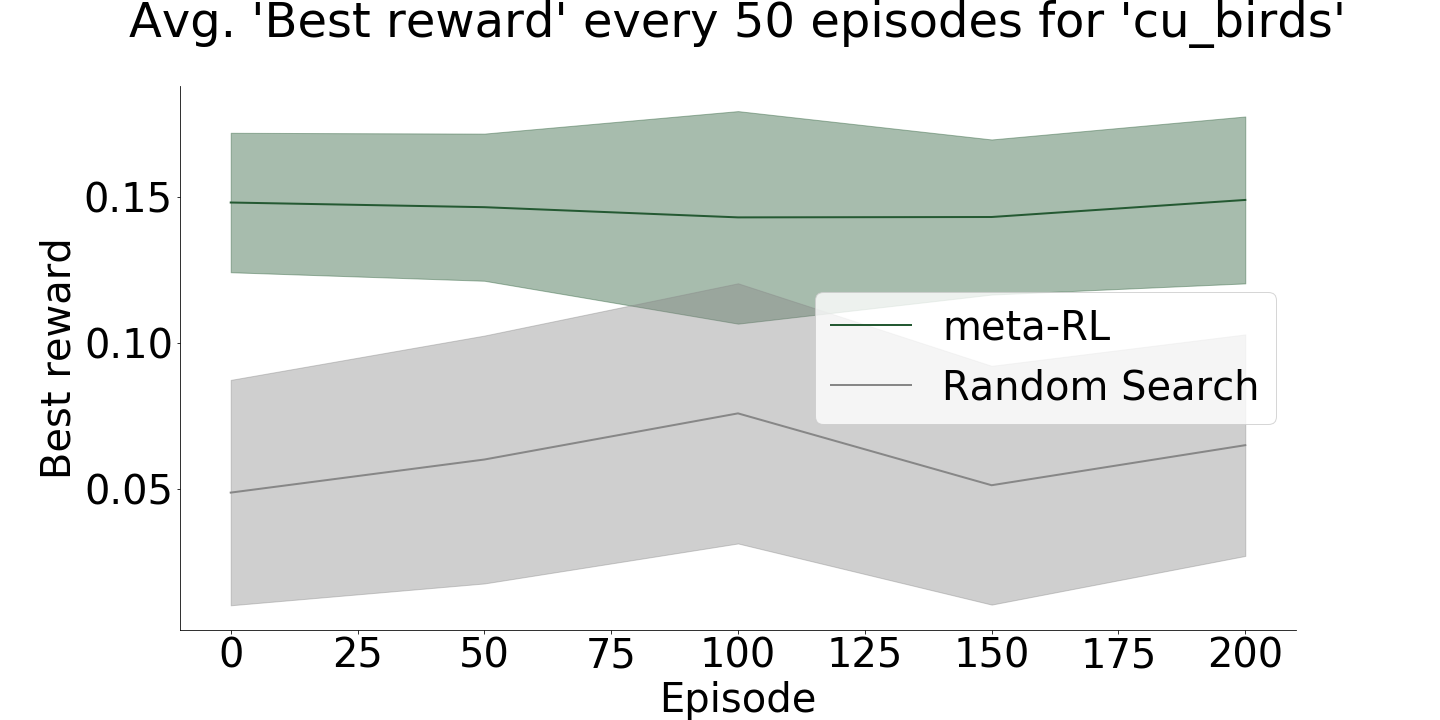
\includegraphics[width=\linewidth]{imgs/chained/average-best_reward-cu_birds.png}
  \caption{} 
\label{fig:results:exp2:evolution:d}
\end{subfigure}%
\begin{subfigure}{.33\textwidth}
  \centering
      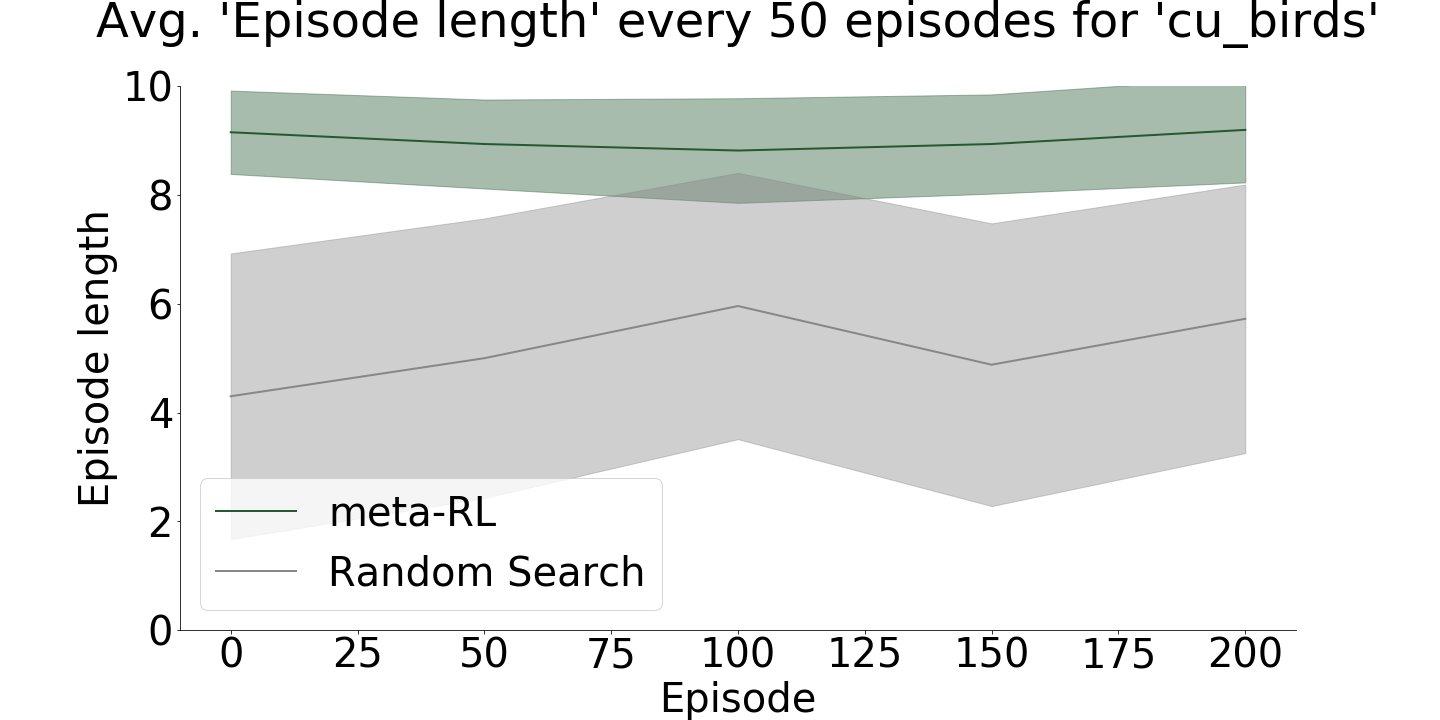
\includegraphics[width=\linewidth]{imgs/chained/average-ep_length-cu_birds.png}
  \caption{}
\label{fig:results:exp2:evolution:e}
\end{subfigure}%
\begin{subfigure}{.33\textwidth}
  \centering
      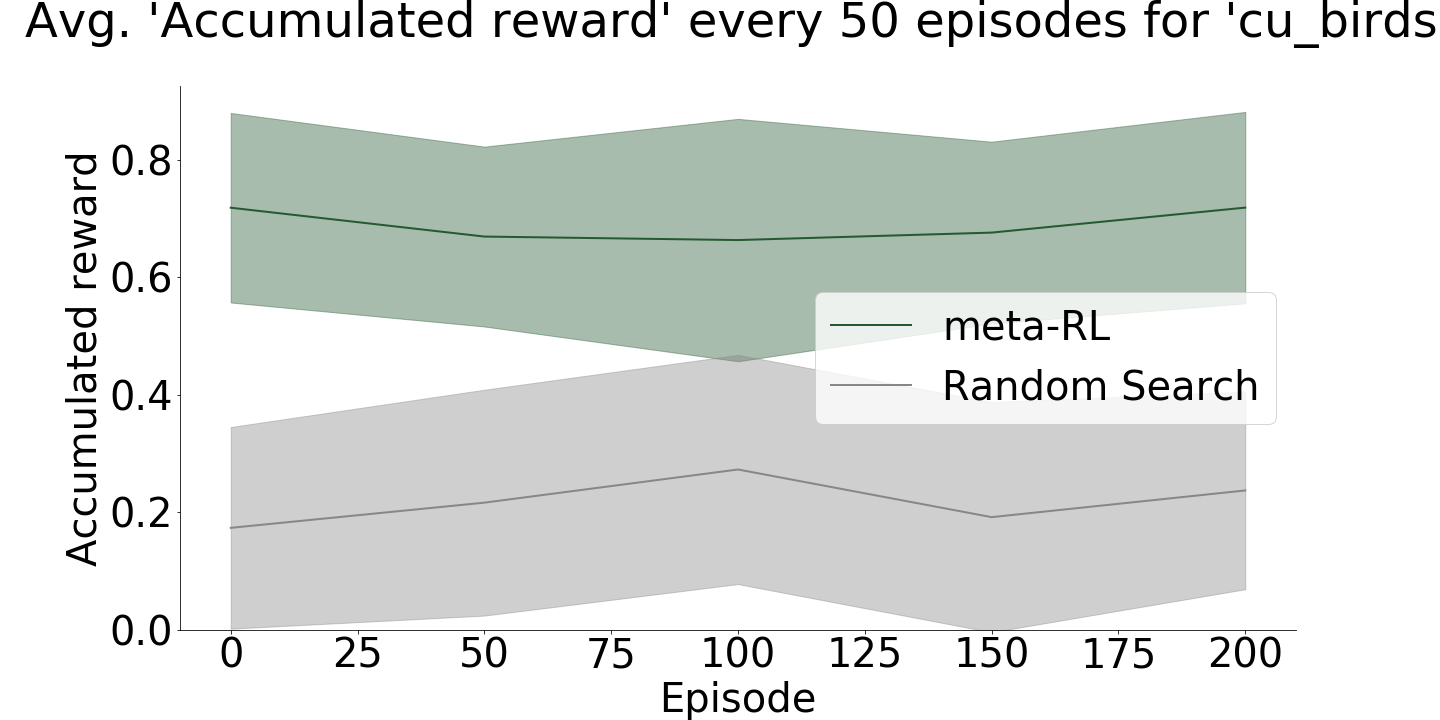
\includegraphics[width=\linewidth]{imgs/chained/average-acc_reward-cu_birds.png}
  \caption{} 
\label{fig:results:exp2:evolution:f}
\end{subfigure}
\caption{Evolution of evaluation episodes through time from different perspectives, showing the means and $\pm 1$ standard deviations for every 50 episodes.}
\label{fig:results:exp2:evolution}
\vspace{-0.5cm}
\end{figure}

\begin{figure}[ht]
\centering
    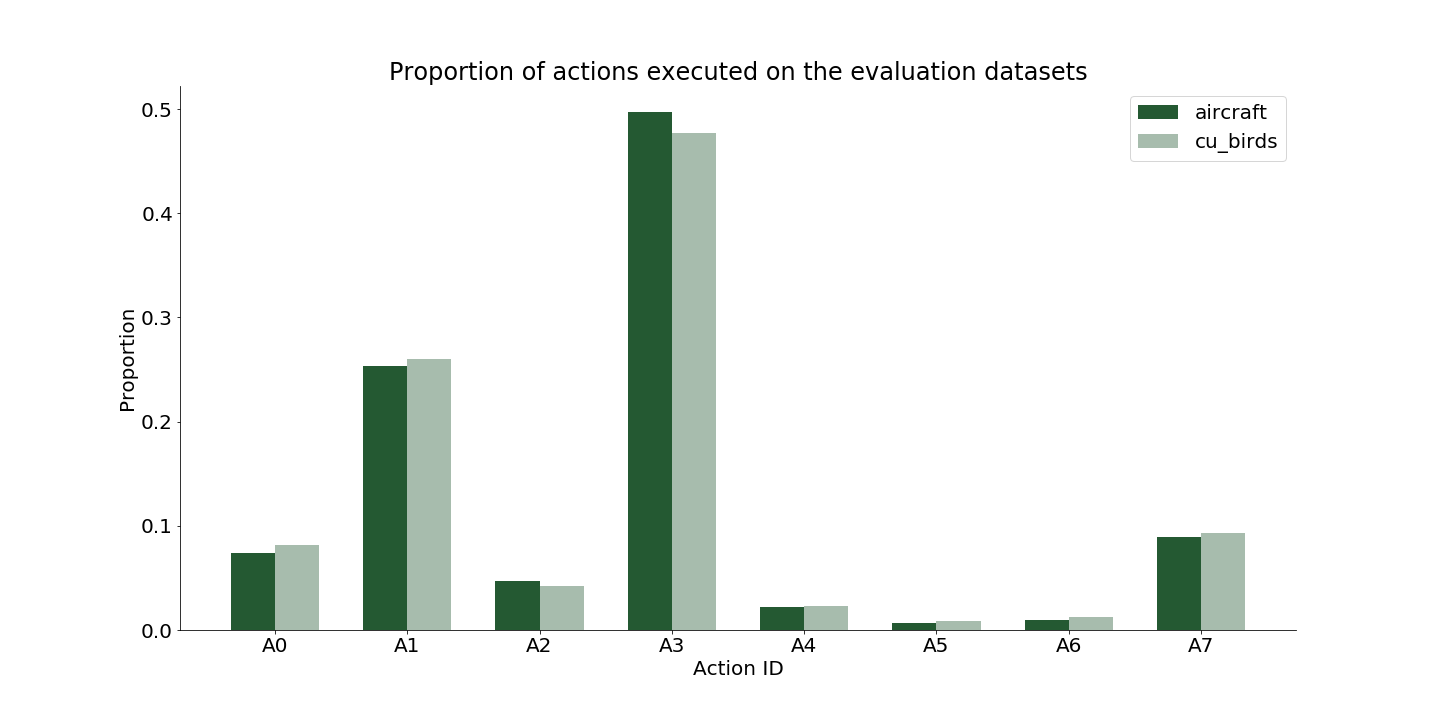
\includegraphics[width=0.85\linewidth]{imgs/chained/actions-dist-evaluation.png}
\caption{Proportion of actions per dataset during evaluation. The labels in the x-axis match the IDs in Table~\ref{tab:methodology:rl:as}.}
\label{fig:results:exp2:actions}
% \vspace{-0.5cm}
\end{figure}

\begin{table}[ht]
\centering
\begin{tabular}{@{}cc@{}}
\toprule
     Dataset             & Runtime \\ \midrule
aircraft  & 2 days 6h   \\
cu\_birds & 2 days 22h  \\ \midrule
Total                    & 5 days 4h  \\ \bottomrule
\end{tabular}
\caption{Running times for the evaluation of the deep meta-RL agent. All experiments ran on a single NVIDIA Tesla K40m GPU.}
\label{tab:results:exp2:times}
\end{table}


As we mentioned in Section~\ref{sec:experiments}, another result of interest is the performance of the best networks designed by the agent when they follow more intensive training. Table~\ref{tab:results:exp2:acc} shows the accuracy values obtained. We note that the networks achieve low accuracy, in the majority of the cases worse than random guessing. An important observation is that these low values can be a consequence of the relaxation made in the shape of the images. Whereas state-of-the-art architectures on both \textit{aircraft} and \textit{cu\_birds} work with shapes greater than $200 \times 200$, we use a smaller version of $84 \times 84$ that might lead to loss of information. Moreover, state-of-the-art results for these datasets are usually obtained after data augmentation and use deeper and more complex networks with multi-branch structures~\citep{FineGrained2, FineGrained3, FineGrainedResults}. However, in this experiment, we do not consider any of the latter aspects since we work under resource constraints that force us to make relaxations, and thus a lower accuracy can be expected.

Despite the low values, the architectures for the two datasets designed by the deep meta-RL agent outperformed by a significant amount the shortened version of VGG19. This shows that by using the learned policy it is possible to find better architectures than one inspired by state-of-the-art networks. A final observation is that the best architecture found by the agent during training did not become the best final network, thus exhibiting that early-stop can underestimate the long-term performance of the networks, which also warrants future work. 

\begin{table}[ht]
\centering
\begin{tabular}{@{}cccc@{}}
\toprule
Dataset   & Deep meta-RL (1st) & Deep meta-RL (2nd)          & VGG19-like                   \\ \midrule
aircraft  & 49.18 $\pm$ 1.2  & \textbf{50.11 $\pm$ 1.02} & 30.85 $\pm$ 10.82 \\
cu\_birds & 23.97 $\pm$ 1.28 & \textbf{24.24 $\pm$ 0.90} & 6.66 $\pm$ 1.98             \\ \bottomrule
\end{tabular}
\caption{Accuracy values of the best architectures after a more intense training. Every reported accuracy value is the mean $\pm$ 2 standard deviations of five independent trainings. For the sake of completeness, we show the designed networks in Appendix~\ref{app:networks}}
\label{tab:results:exp2:acc}
\end{table}

\subsection*{Experiment 3: training on a more complex environment}

Figure~\ref{fig:results:exp3:evolution} shows the evolution of the \textit{best reward}, \textit{episode length}, and \textit{accumulated reward} during the multi-branch experiment on \textit{omniglot}. We do not observe differences in the behavior of the agent when using different $\sigma$ values, but we note that it took longer to output meaningful rewards (around episode 3000) when compared to Experiment 1, causing extended runtimes as shown in Table~\ref{tab:results:exp3:times}.

\begin{figure}[ht]
\centering
\begin{subfigure}{.40\textwidth}
  \centering
      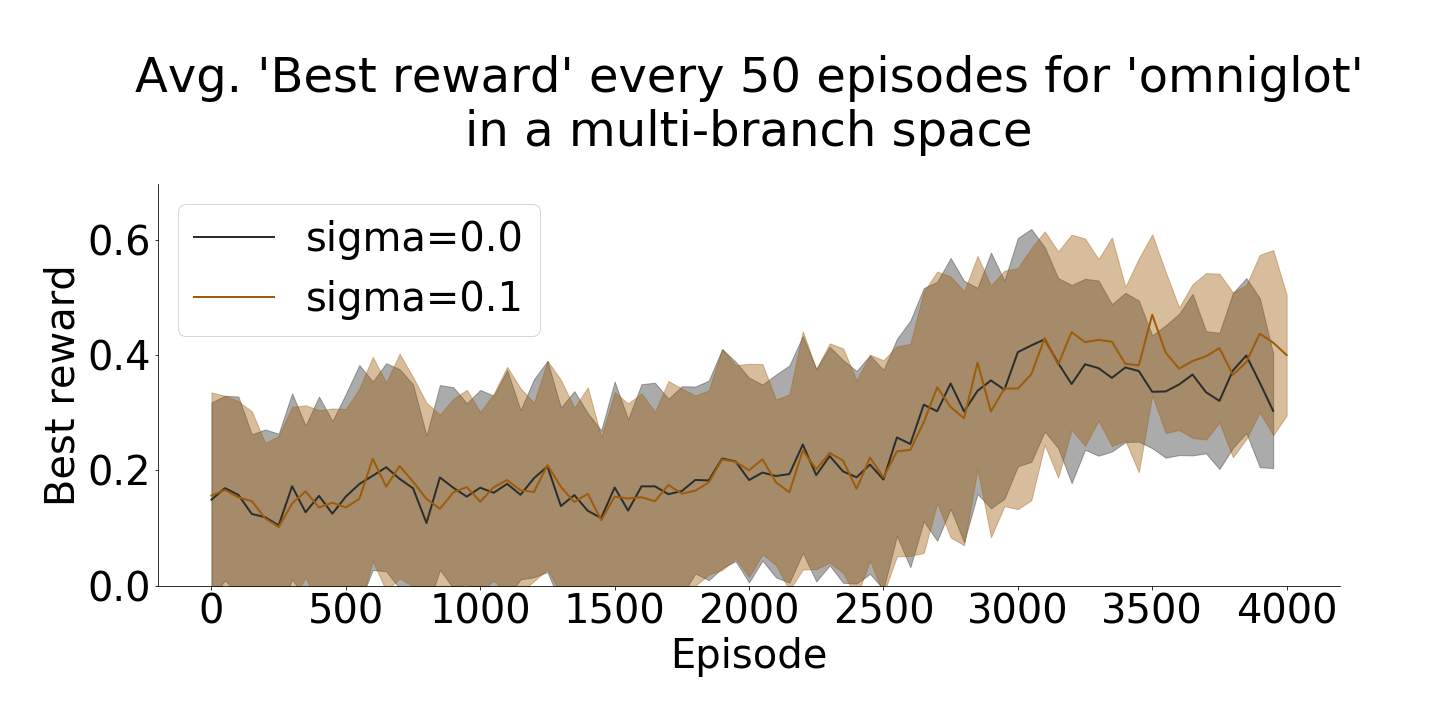
\includegraphics[width=\linewidth]{imgs/multibranch/average-best_reward-omniglot.png}
  \caption{}
  \label{fig:results:exp3:evolution:a}
\end{subfigure}%
\begin{subfigure}{.40\textwidth}
  \centering
      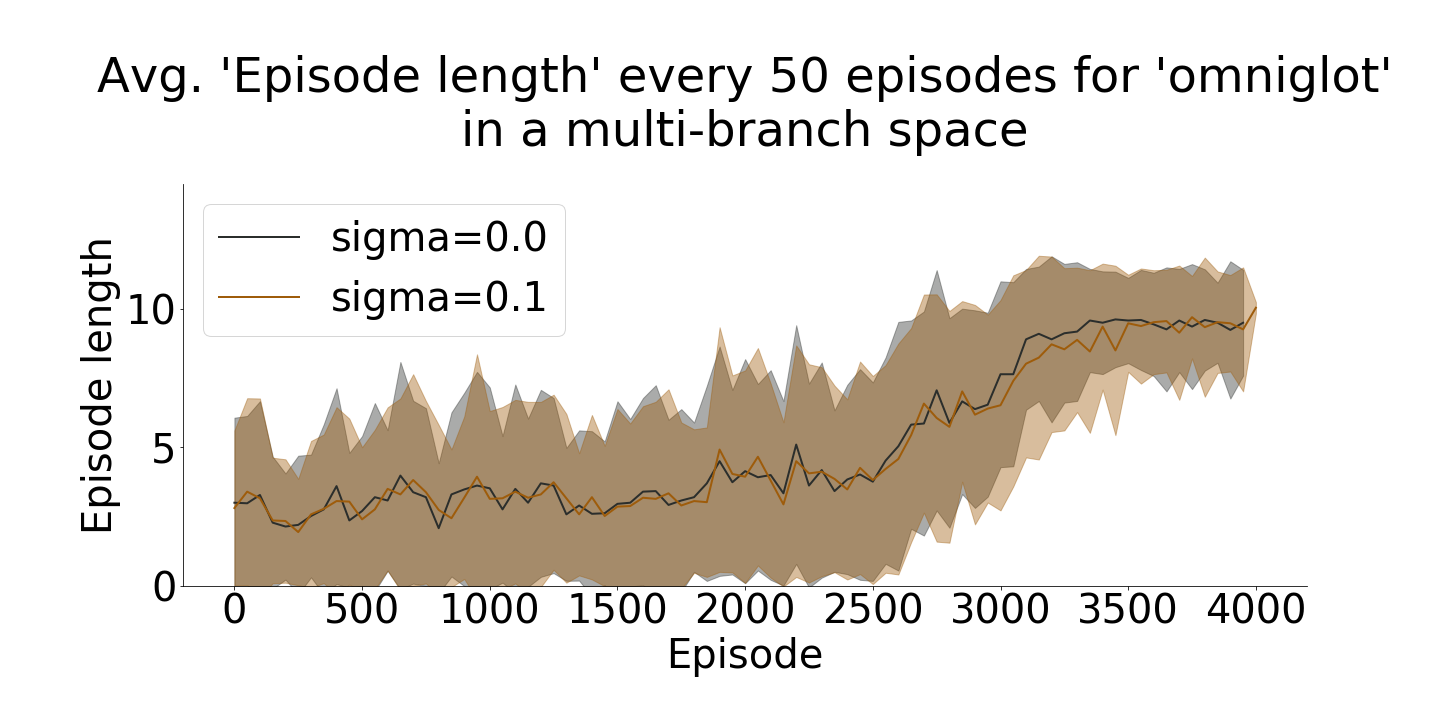
\includegraphics[width=\linewidth]{imgs/multibranch/average-ep_length-omniglot.png}
  \caption{}
  \label{fig:results:exp3:evolution:b}
\end{subfigure}
\begin{subfigure}{.40\textwidth}
  \centering
      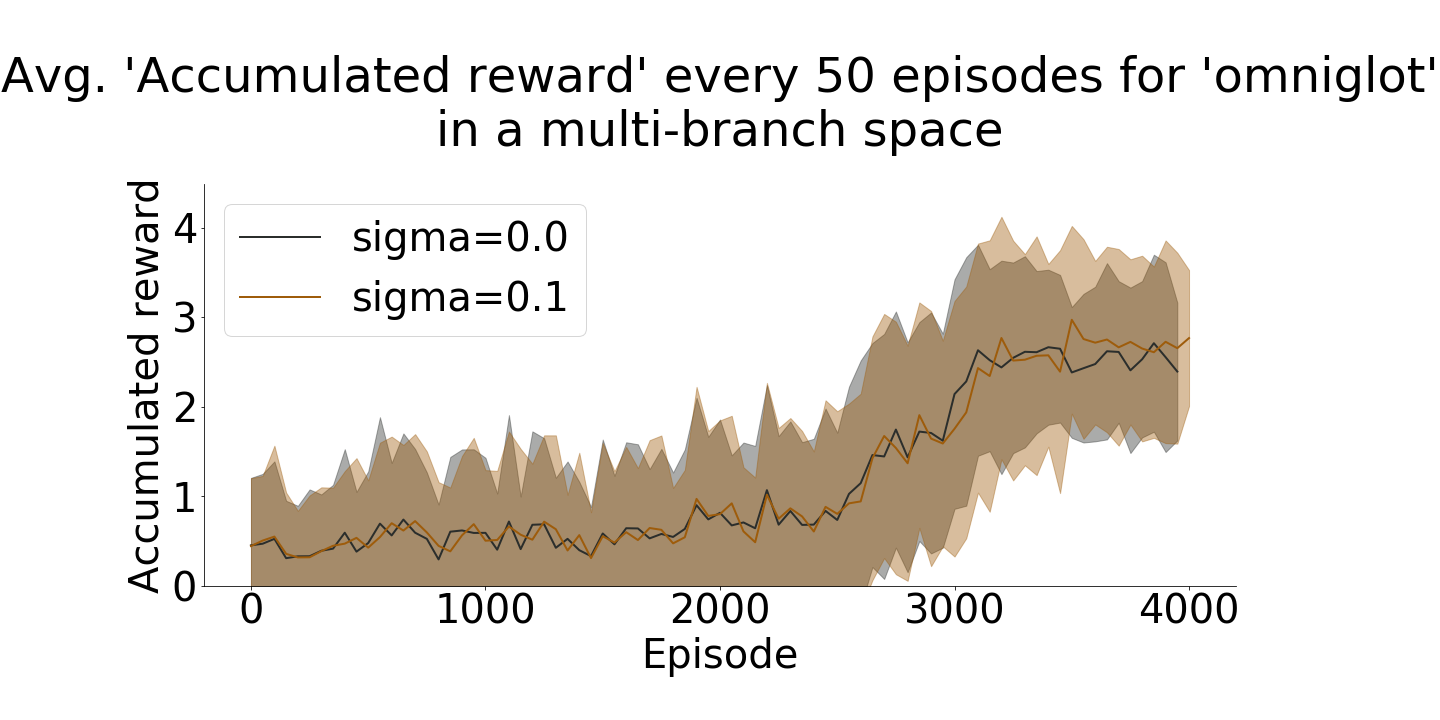
\includegraphics[width=\linewidth]{imgs/multibranch/average-acc_reward-omniglot.png}
  \caption{}
\label{fig:results:exp3:evolution:c}
\end{subfigure}
\caption{Evolution of training episodes for the multi-branch experiment from different perspectives. The plots show the means and $\pm 1$ standard deviations for every 50 episodes.}
\label{fig:results:exp3:evolution}
\vspace{-0.5cm}
\end{figure}

\begin{table}[ht]
\centering
\begin{tabular}{@{}cc@{}}
\toprule
                  & Runtime \\ \midrule
$\sigma = 0.0$ & 13 days 9h   \\
$\sigma = 0.1$ & 15 days 14h  \\ \midrule
Total                    & 28 days 23h  \\ \bottomrule
\end{tabular}
\caption{Runtimes for the training of the deep meta-RL agent in the multi-branch search space for \textit{omniglot}. All experiments ran on a single NVIDIA Tesla K40m GPU.}
\label{tab:results:exp3:times}
\end{table}


However, we stated in Section~\ref{sec:experiments:multibranch} that our main interest in this experiment is to study whether or not the agent can explore multi-branch structures. Figure~\ref{fig:results:exp3:exploration:a} shows the entropy of the policy through time-steps, and Figure~\ref{fig:results:exp3:exploration:b} the count of multi-branch structures through episodes. We note that during exploration the appearance of multi-branch structures is more likely, and after episode 3000 (represented by the vertical line in Figure~\ref{fig:results:exp3:exploration:a}), when exploration drops down, the multi-branch structures become less frequent. Furthermore, we found that the proportion of multi-branch vs.~chain-structured networks is only 1:10, meaning that the agent did not explore multi-branch structures aggressively, and settled for chain-structured networks instead. The latter is supported by the proportion of actions displayed in Figure~\ref{fig:results:exp3:actions}, where the actions \textsc{A8-13} (related to multi-branch structures) are the least frequent.



\begin{figure}[ht]
\centering
\begin{subfigure}{.53\textwidth}
  \centering
      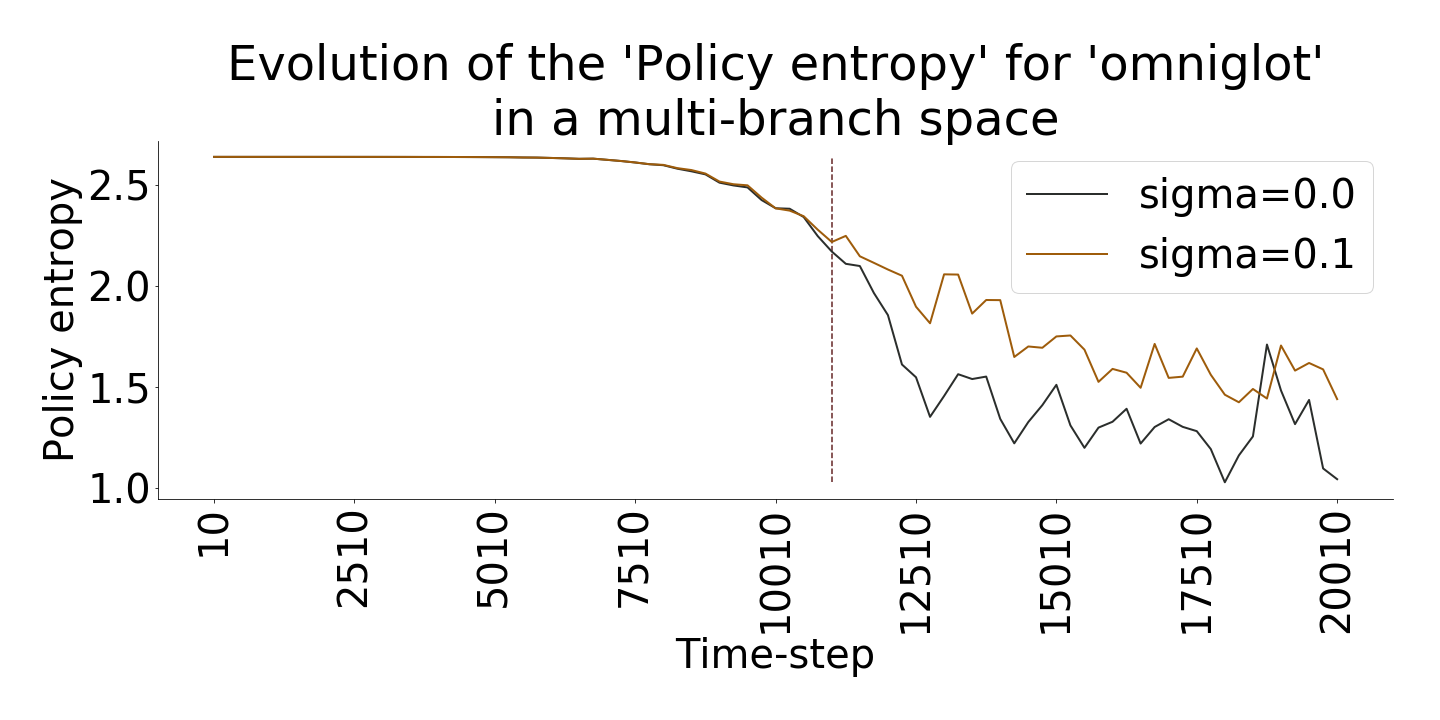
\includegraphics[width=\linewidth]{imgs/multibranch/entropy.png}
  \caption{}
  \label{fig:results:exp3:exploration:a}
\end{subfigure}%
\begin{subfigure}{.44\textwidth}
  \centering
      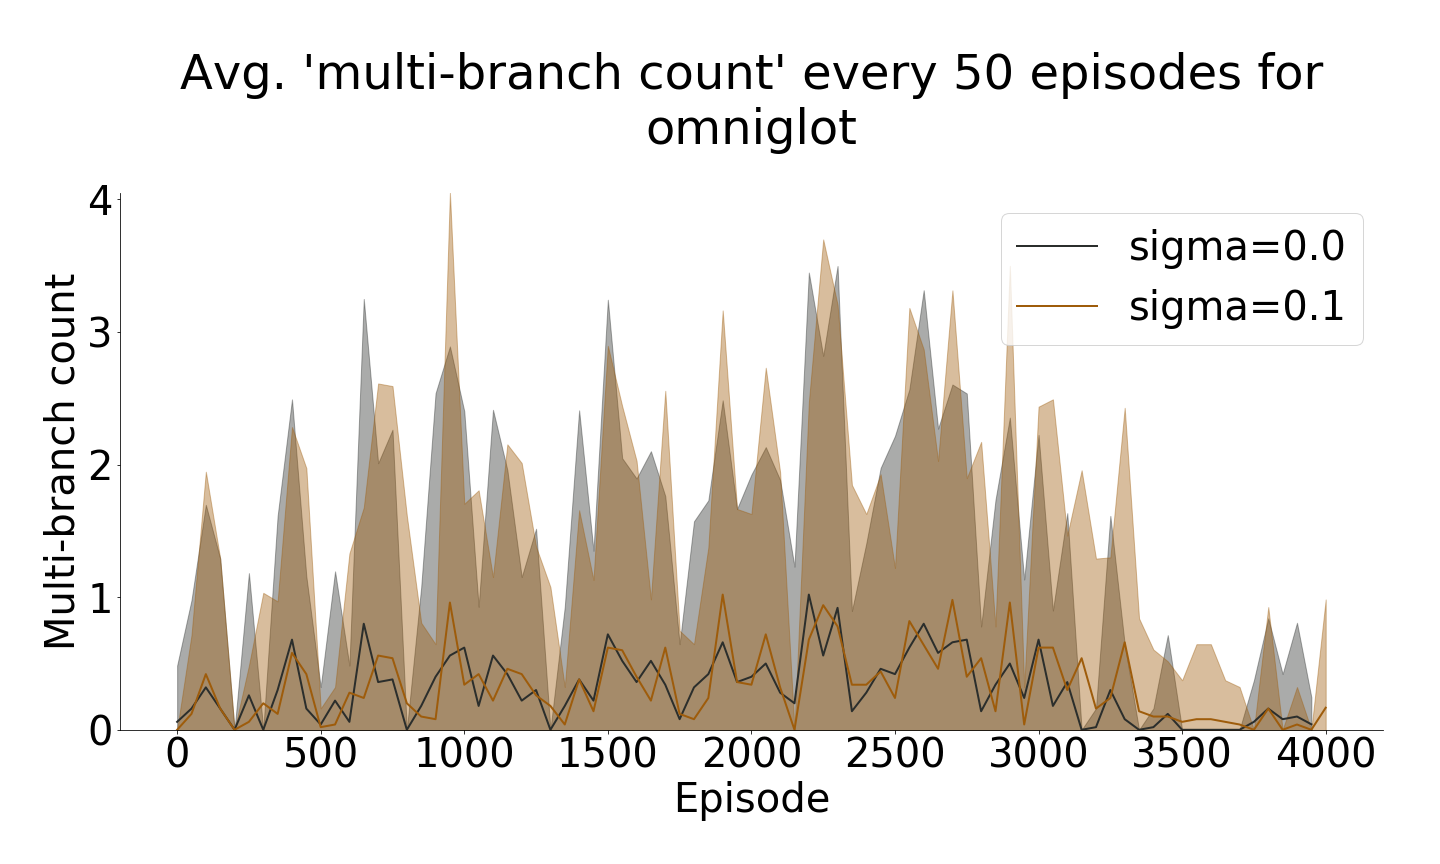
\includegraphics[width=\linewidth]{imgs/multibranch/average-mb_count-omniglot.png}
  \caption{}
  \label{fig:results:exp3:exploration:b}
\end{subfigure}
\caption{The exploration of the agent through time. (a) The entropy of the policy through time-steps. The vertical line cuts the horizontal axis at the time-step where the episde 3000 starts. (b) The count of multi-branch structures explored by the agent, showing the mean $\pm$ 1 standard deviation every 50 episodes.\\}
\label{fig:results:exp3:exploration}
\vspace{-0.5cm}
\end{figure}


\begin{figure}[ht]
\centering
    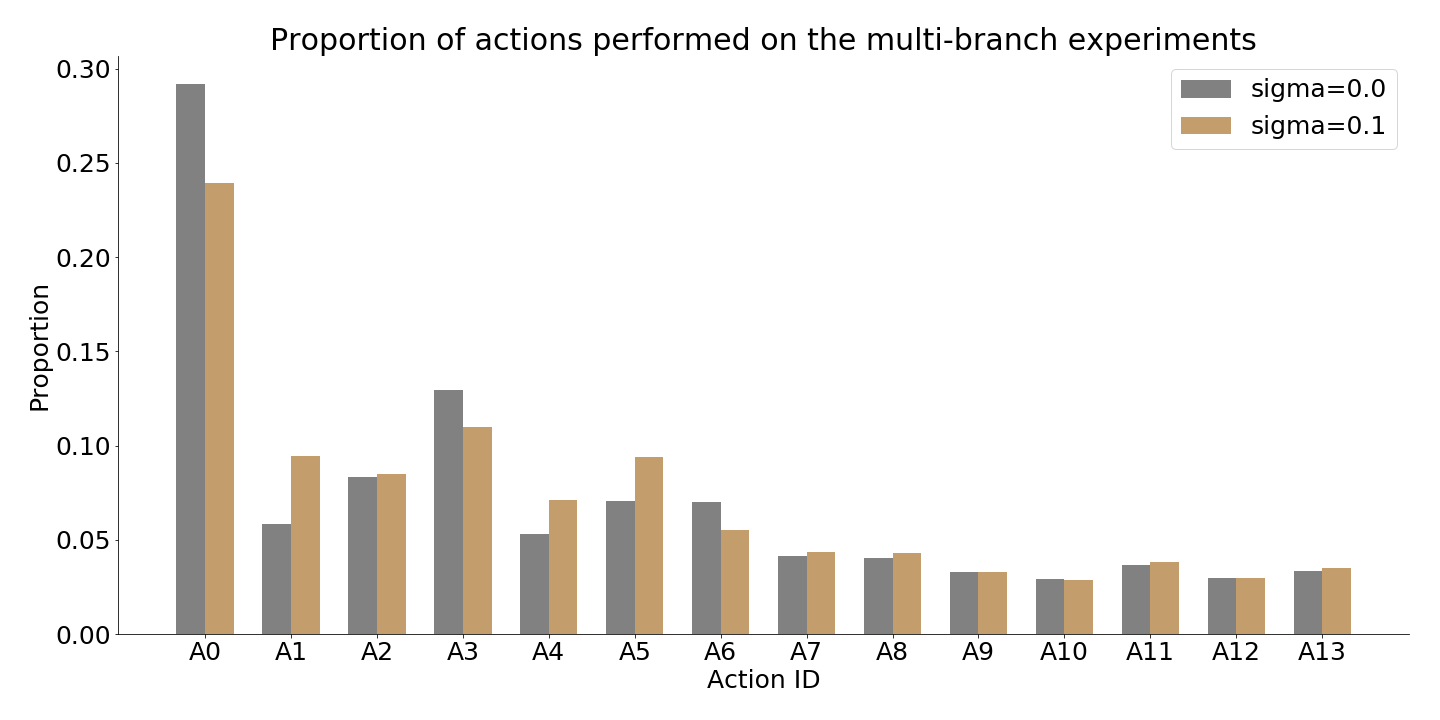
\includegraphics[width=0.65\linewidth]{imgs/multibranch/actions-dist-mb.png}
\caption{Proportion of actions taken by the agent in the multi-branch experiments. The labels in the x-axis match the IDs in Table~\ref{tab:methodology:rl:as}.}
\label{fig:results:exp3:actions}
% \vspace{-0.5cm}
\end{figure}

We believe that a multi-branch space requires us to handle differently how the predecessors of the NSC vectors are selected (see Section~\ref{sec:methodology:rl:as}). Some alternatives are: defining heuristics to chose the predecessors instead of using the shifting operations, assigning other rewards to the actions related to the predecessors, and modifying the hyper-parameters of the A2C network to encourage more exploration of the agent in the beginning of the deep meta-RL training.
